\documentclass[tikz,dvisvgm,border=1pt]{standalone}
% Shared preamble for the attribution infographics (iN-*.tex).
% tools/tikz-build.sh compiles each source with \variant set to wide or narrow.
\usepackage[T1]{fontenc}
\usepackage[default,semibold]{sourcesanspro}
\usepackage[italic]{mathastext}
% Larger scripts than the TeX default, so subscripts stay legible at phone width.
\DeclareMathSizes{9}{9}{8}{7}
\DeclareMathSizes{10}{10}{9}{8}
\DeclareMathSizes{11}{11}{9}{8}
\DeclareMathSizes{11.5}{11.5}{9.5}{8}
\usetikzlibrary{arrows.meta,positioning,calc,fit,backgrounds,decorations.pathreplacing,patterns}

\ifdefined\variant\else\def\variant{wide}\fi
\newif\ifnarrow
\def\narrowname{narrow}
\ifx\variant\narrowname\narrowtrue\fi
% The narrow variant is about 320pt wide and shown at about 350px, the wide one
% about 540pt wide and shown at up to 720px: the narrow one uses larger type.
\ifnarrow
  \def\basefont{\fontsize{11}{13}\selectfont}\def\smallfont{\fontsize{10}{12}\selectfont}
  \def\titlefont{\fontsize{11.5}{13.5}\selectfont\bfseries}
\else
  \def\basefont{\fontsize{10}{12}\selectfont}\def\smallfont{\fontsize{9}{11}\selectfont}
  \def\titlefont{\fontsize{11}{13}\selectfont\bfseries}
\fi

% Light-theme page tokens (web/src/styles/_variables.css, embeds.css), fixed:
% every infographic sits on its own light card, so it reads on both themes.
\definecolor{ink}{HTML}{262626}      % --text-color on white
\definecolor{muted}{HTML}{666666}    % --muted-color on white
\definecolor{rule}{HTML}{DCDCDC}     % --border-color, slightly stronger
\definecolor{surface}{HTML}{F5F5F5}  % --neutral-200
\definecolor{heading}{HTML}{904B20}  % h2 colour
\definecolor{info}{HTML}{187C9B}     % embeds --info-color
\definecolor{primary}{HTML}{C65928}  % embeds --primary-color
\definecolor{success}{HTML}{35814C}  % embeds --success-color
\definecolor{danger}{HTML}{BD3F50}   % f13 spread cost
\definecolor{residual}{HTML}{A77913} % f13 residual

\tikzset{
  every picture/.style={color=ink, line width=0.6pt, >={Stealth[length=5pt,width=4pt]},
    font=\basefont},
  small/.style={font=\smallfont},
  title/.style={font=\titlefont},
  box/.style={draw=rule, fill=white, rounded corners=4pt, align=center, inner sep=5pt},
  tag/.style={small, text=muted},
}

% No hyphenation in the narrow text columns of the diagrams.
\hyphenpenalty=10000 \exhyphenpenalty=10000

% Light card behind the whole drawing, below the background layer.
\pgfdeclarelayer{card}
\pgfsetlayers{card,background,main}
\newcommand\drawcard{%
  \begin{pgfonlayer}{card}
    \fill[white, draw=rule, rounded corners=8pt]
      ($(current bounding box.south west)+(-10pt,-10pt)$)
      rectangle ($(current bounding box.north east)+(10pt,10pt)$);
  \end{pgfonlayer}}

% Section 4: two indicators share information about an outcome; the same
% Shapley rule shares it, and the chosen game v(S) fixes what the shares mean.
\begin{document}
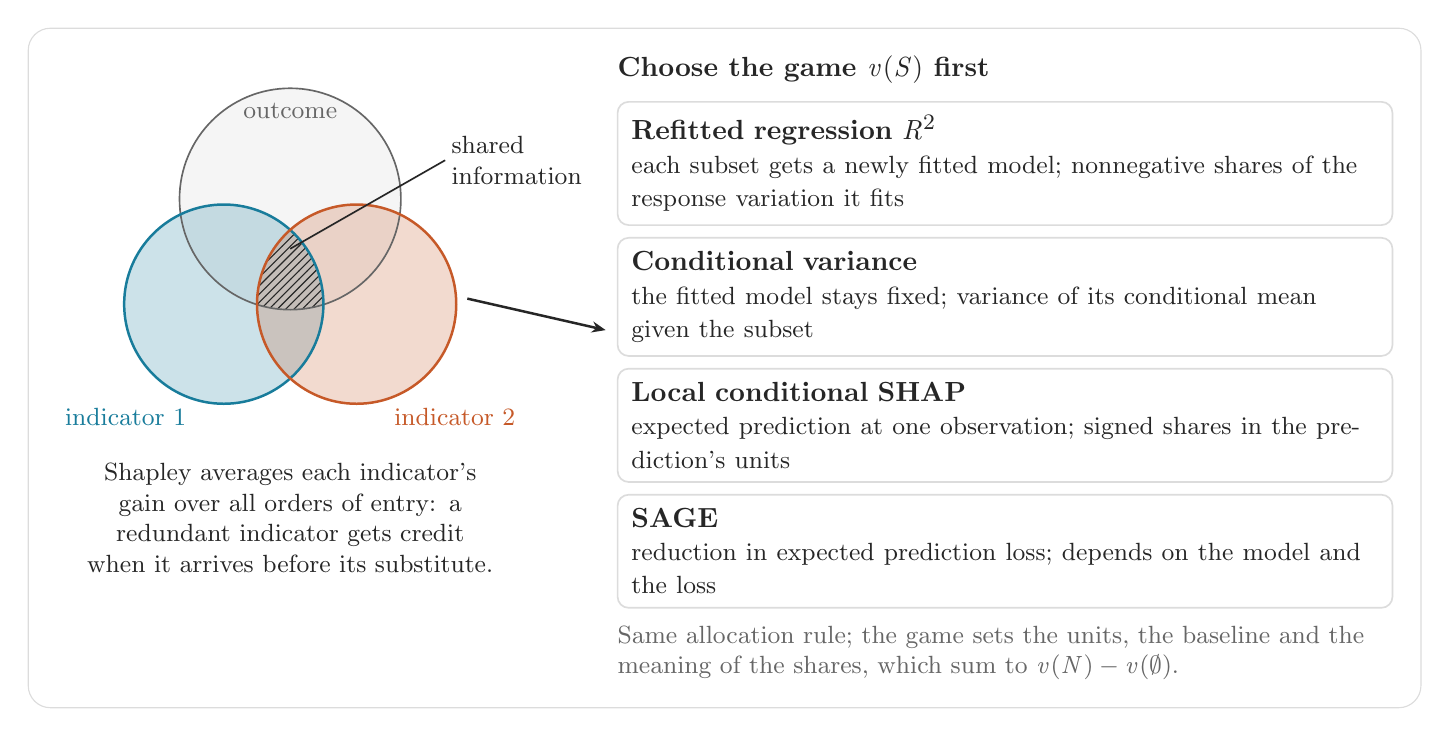
\begin{tikzpicture}[
  game/.style={box, align=left, inner sep=5pt},
]
\ifnarrow
  \def\gamew{262pt}\def\venn{(0,0)}
\else
  \def\gamew{270pt}
\fi
% Venn: outcome Y and two correlated indicators.
\def\Y{(0,26pt) circle (40pt)}
\def\A{(-24pt,-12pt) circle (36pt)}
\def\B{(24pt,-12pt) circle (36pt)}
\fill[surface] \Y;
\fill[info, fill opacity=0.22] \A;
\fill[primary, fill opacity=0.22] \B;
\begin{scope}
  \clip \Y; \clip \A; \clip \B;
  \fill[pattern=north east lines, pattern color=ink] (-60pt,-60pt) rectangle (60pt,80pt);
\end{scope}
\draw[muted] \Y; \draw[info, line width=0.9pt] \A; \draw[primary, line width=0.9pt] \B;
\node[small, text=muted] at (0,58pt) {outcome};
\node[small, text=info, anchor=north east] at (-34pt,-46pt) {indicator 1};
\node[small, text=primary, anchor=north west] at (34pt,-46pt) {indicator 2};
\draw[ink] (0,8pt) -- (56pt,40pt) node[right, small, align=left, inner sep=2pt] {shared\\information};
\node[small, text width=150pt, align=center, anchor=north] (rule) at (0,-66pt) {%
  Shapley averages each indicator's gain over all orders of entry: a redundant
  indicator gets credit when it arrives before its substitute.};

% The games.
\ifnarrow
  \node[anchor=north west, inner sep=0pt, font=\basefont\bfseries] (gt) at ($(rule.south)+(-131pt,-14pt)$)
    {Choose the game $v(S)$ first};
\else
  \node[anchor=north west, inner sep=0pt, font=\basefont\bfseries] (gt) at (118pt,78pt)
    {Choose the game $v(S)$ first};
\fi
\node[game, text width=\gamew, anchor=north west] (g1) at ($(gt.south west)+(0,-6pt)$)
  {\textbf{Refitted regression $R^2$}\\{\smallfont each subset gets a newly fitted model;
   nonnegative shares of the response variation it fits}};
\node[game, text width=\gamew, below=4pt of g1] (g2)
  {\textbf{Conditional variance}\\{\smallfont the fitted model stays fixed; variance of its
   conditional mean given the subset}};
\node[game, text width=\gamew, below=4pt of g2] (g3)
  {\textbf{Local conditional SHAP}\\{\smallfont expected prediction at one observation;
   signed shares in the prediction's units}};
\node[game, text width=\gamew, below=4pt of g3] (g4)
  {\textbf{SAGE}\\{\smallfont reduction in expected prediction loss; depends on the model
   and the loss}};
\node[anchor=north west, inner sep=0pt, small, text=muted, text width=\gamew]
  at ($(g4.south west)+(0,-6pt)$) {Same allocation rule; the game sets the units, the
  baseline and the meaning of the shares, which sum to $v(N)-v(\emptyset)$.};
\ifnarrow\else
  \draw[->, line width=0.9pt] (64pt,-10pt) -- ($(g2.west)+(-4pt,-12pt)$);
\fi
\drawcard
\end{tikzpicture}
\end{document}
